\documentclass[10pt,twocolumn]{IEEEtran}
% \documentclass[12pt, draftcls, onecolumn]{IEEEtran}
\makeatletter
\def\subsubsection{\@startsection{subsubsection}
                                 {3}
                                 {\z@}
                                 {0ex plus 0.1ex minus 0.1ex}
                                 {0ex}
                             {\normalfont\normalsize\bfseries}}
\makeatother
\usepackage[T1]{fontenc}
\usepackage{subfigure}
\usepackage{ulem}
\usepackage{amsmath}
\allowdisplaybreaks
\usepackage{hhline}
\usepackage{graphicx}
\usepackage{yfonts,color}
\usepackage{soul,xcolor}
\usepackage{verbatim}
\usepackage{amsmath}
\allowdisplaybreaks
\usepackage{amssymb}
\usepackage{amsthm}
\usepackage{float}
\usepackage{bm}
\usepackage{url}
\usepackage{array}
\usepackage{cite}
\usepackage{tikz}
\usepackage{framed}
\usepackage{balance}
\usepackage{epsfig,epstopdf}
\usepackage{booktabs}
\usepackage{courier}
\usepackage{subfigure}
\usepackage{pseudocode}
\usepackage{enumerate}
\usepackage{algorithm}
\usepackage{algpseudocode}
\newtheorem{definition}{Definition}
\newtheorem{theorem}{Theorem}
\newtheorem{lemma}[theorem]{Lemma}
\newtheorem{proposition}[theorem]{Proposition}
\newtheorem{corollary}[theorem]{Corollary}
\newtheorem{assumption}{Assumption}
\newtheorem{remark}{Remark}
\renewcommand{\algorithmicrequire}{\textbf{Initialization:}}  
\renewcommand{\algorithmicensure}{\textbf{Output:}}  
\newcommand{\rom}[1]{\uppercase\expandafter{\romannumeral #1\relax}}
\usepackage{color}
\usepackage{soul,xcolor}
\newcommand{\sst}[1]{\st{#1}}
%\newcommand{\sst}[1]{}
\newcommand{\nm}[1]{{\color{blue}\bf{[NM: #1]}}}
%\newcommand{\nm}[1]{}
\newcommand{\bk}[1]{{\color{magenta}{[BK: #1]}}}
\newcommand{\nmmath}[1]{{\color{blue}\text{\bf{[NM: #1]}}}}
\newcommand{\gs}[1]{{\color{orange}\bf{[GS: #1]}}}
\newcommand{\remove}[1]{{\color{magenta}{\bf REMOVE: [#1]}}}
\DeclareMathOperator*{\argmax}{arg\,max}
\DeclareMathOperator*{\argmin}{arg\,min}
\usepackage{cancel}
\newcommand\mst[2][red]{\setbox0=\hbox{$#2$}\rlap{\raisebox{.45\ht0}{\textcolor{#1}{\rule{\wd0}{2pt}}}}#2} 
%\newcommand{\mst}[1]{} 
\newcommand{\add}[1]{{\color{red}{#1}}}
\newcommand{\ull}[1]{\textbf{\color{red}\ul{#1}}}
\renewcommand{\baselinestretch}{0.96}
\normalem
\title{Spectrum Sensing in Cognitive Radio Networks
\\
via Approximate POMDP}
\author{Bharath Keshavamurthy, Nicol\`{o} Michelusi
\thanks{This research has been funded in part by NSF under grant CNS-1642982.}
\thanks{The authors are with the School of Electrical and Computer Engineering, Purdue University. email: \{bkeshava,michelus\}@purdue.edu.}
\vspace{-12mm}}
\begin{document}
\maketitle
\thispagestyle{empty}
\pagestyle{empty} 
\setulcolor{red}
\setul{red}{2pt}
\setstcolor{red}
\begin{abstract}
In this letter, a novel spectrum sensing and access strategy based on POMDPs is proposed. A cognitive radio learns the correlation model defining the occupancy behavior of incumbents, based on which it devises an optimal sensing and access policy. The optimization complexity is ameliorated via point-based value iteration methods. Numerical evaluations demonstrate that the proposed framework achieves higher throughput for cognitive radios, with lower interference to incumbents, compared to state-of-the-art clustering algorithms and a Neyman-Pearson detector that assumes independence among channels. Furthermore,\sst{ the proposed scheme} \add{it} achieves performance comparable to\sst{ that of} HMM MAP estimators\sst{ which possess} \add{with} a priori knowledge of the correlation model.
\end{abstract}
\begin{IEEEkeywords}
Hidden Markov Model, Cognitive Radio, Spectrum Sensing, POMDP
\end{IEEEkeywords}
\vspace{-4mm}
\section{Introduction}\label{I}
The advent of fifth-generation wireless communication networks has exacerbated the problem of spectrum scarcity \cite{7158089}. Cognitive radio networks facilitate efficient spectrum utilization by intelligently accessing \emph{white spaces} left unused by the sparse and infrequent transmissions of licensed users, while ensuring incumbent non-interference compliance \cite{4562537}. 

A crucial aspect underlying the design of cognitive radio networks is the ability to perform spectrum sensing. However, physical design limitations are imposed on the cognitive radio's spectrum sensor in view of quick turnaround times and energy efficiency \cite{5990482}, which restrict the number of channels that can be sensed at any given time. This has led to research in algorithms that first determine the best channels to sense\sst{, after which the gathered information is used to perform} \add{before making} channel access decisions. The state-of-the-art are based on multi-armed bandits \cite{7094730}, reinforcement learning \cite{6507570}, and custom heuristics \cite{4554696, 6956794}. However, most of these works, such as \cite{7094730, 6507570, 7895211, 7336513, 8571293}, assume independence across frequency bands, which is imprudent because licensed users may exhibit correlations across both frequency and time in their channel occupancy behavior: they may occupy a set of adjacent frequency bands for an extended period of time \cite{6188346}. This correlation structure may be leveraged for more accurate predictions of spectrum holes. In this letter, we propose a parameter estimation algorithm to learn the frequency and time correlation structure, based on which we solve for the optimal sensing and access policy via partially observable Markov decision processes (POMDPs).

\noindent {\bf Related Work:}
Distributed spectrum sensing has been considered in \cite{6507570} and solved using SARSA with linear value function approximation. However, frequency correlation is precluded, and errors in state estimation are neglected in the decision process. In \cite{6956794}, the frequency correlation is exploited, but\sst{ a noise-free} \add{the} observation model is\sst{ assumed} \add{noise-free}. Compared to \cite{6507570, 6956794}, we account for the uncertainty in the occupancy state and for noisy observations via a POMDP formulation. Standard MAP-based state estimators for Hidden Markov Models (HMMs) such as the Viterbi algorithm can be employed to estimate spectrum occupancy \cite{4554696}; however, these estimators rely on knowledge of the transition model, which may be unknown in practice. To this end, in \cite{6956794, 4554696}, the time-frequency correlation structure is estimated offline based on pre-loaded databases. However, this solution may be impractical in non-stationary settings. To fill this gap, in our work, we develop a fully online framework  to learn the parametric time-frequency correlation model, and embed it directly into the sensing and access optimization and decision engine. It is also worth noting that \cite{4554696} does not impose sensing restrictions on the cognitive radio, as we do. Finally, unlike\sst{ other related works in the state-of-the-art} \cite{7094730, 6507570, 4554696, 6956794}, our POMDP framework\sst{ facilitates the regulation of} \add{allows to regulate} the trade-off between the throughput achieved by the cognitive radio and the interference to the incumbents.

In a nutshell, the contributions of this paper are as follows:
we develop a POMDP framework for spectrum sensing and access in a radio environment with multiple licensed users exhibiting correlations in their occupancy behavior across both time and frequency, assuming a linear, Gaussian observation model with sensing limitations; we develop an online parameter estimation algorithm to learn the incumbents' occupancy correlation model; 
concurrently, we propose a randomized point-based value iteration algorithm\sst{ that solves the POMDP formulation for} \add{to find} the optimal spectrum sensing and access policy;\sst{ and} finally, we compare  \add{numerically} the proposed framework with state-of-the-art algorithms, and demonstrate superior performance. The rest of the paper is organized as follows: in Sec. \ref{II}, we define the system model, followed by the formulations, approaches, and algorithms in Sec. \ref{III}; in Sec. \ref{IV}, we present numerical evaluations, followed by our conclusions in Sec. \ref{V}.
\vspace{-3mm}
\section{System Model}\label{II}
\noindent {\bf Signal Model:}
We consider a network\sst{ consisting} of $J$ incumbents\sst{ termed the Primary Users} (\add{Primary Users, }PUs) and one cognitive radio\sst{ termed the Secondary User} (\add{Secondary User,} SU) equipped with a spectrum sensor. The goal of the SU is to maximize its own throughput by opportunistically accessing portions of the spectrum left unused by the PUs. To this end, the SU should learn how to intelligently access spectrum holes, while ensuring nominal interference with incumbent transmissions.
We express the discretized wideband frequency domain signal received at the SU as
\begin{equation}\label{2}
    Y_k(i) = \sum_{j=1}^{J} H_{j,k}(i)X_{j,k}(i) + V_k(i),
\end{equation}
where $i {\in} \{1,2\mst{,3},\dots,T\}$ represents the time index; $k {\in} \{1,2\mst{,3},\dots,K\}$
is the frequency domain channel index; $X_{j,k}(i)$ is the signal of the $j$th PU in the frequency domain, and $H_{j,k}(i)$ is the frequency domain channel between the $j$th PU and the SU; $V_k(i) {\sim} \mathcal{CN}(0,\sigma_V^2)$ represents circularly symmetric additive complex Gaussian noise, i.i.d across frequency and across time, and independent of channel $H$ and PU signal $X$. We further assume that the $J$ PUs employ an orthogonal \add{spectrum} access\sst{ to the spectrum} (e.g., OFDMA) so that $X_{j,k}(i)X_{g,k}(i){=}0, \forall j{\neq}g$. Thus, letting $j_{k,i}$ be the index of the PU that occupies the $k$th spectrum band at time $i$, and letting  $H_{k}(i){=}H_{j_{k,i},k}(i)$ and $X_{k}(i){=}X_{j_{k,i},k}(i)$ (with $X_{k}(i){=}0$, if no PU is transmitting in the $k$th spectrum band at time $i$), we can rewrite \eqref{2} as 
\begin{equation}\label{3}
    Y_k(i) = H_{k}(i)X_{k}(i) + V_k(i).
\end{equation}
We model the channel as Rayleigh fading, so that $H_{k}(i)$ is a zero-mean circularly symmetric complex Gaussian random variable with variance $\sigma_H^2$, $H_k {\sim} \mathcal{CN}(0,\sigma_H^2)$, i.i.d. across frequency bands and time.
\begin{figure}
    \centering
    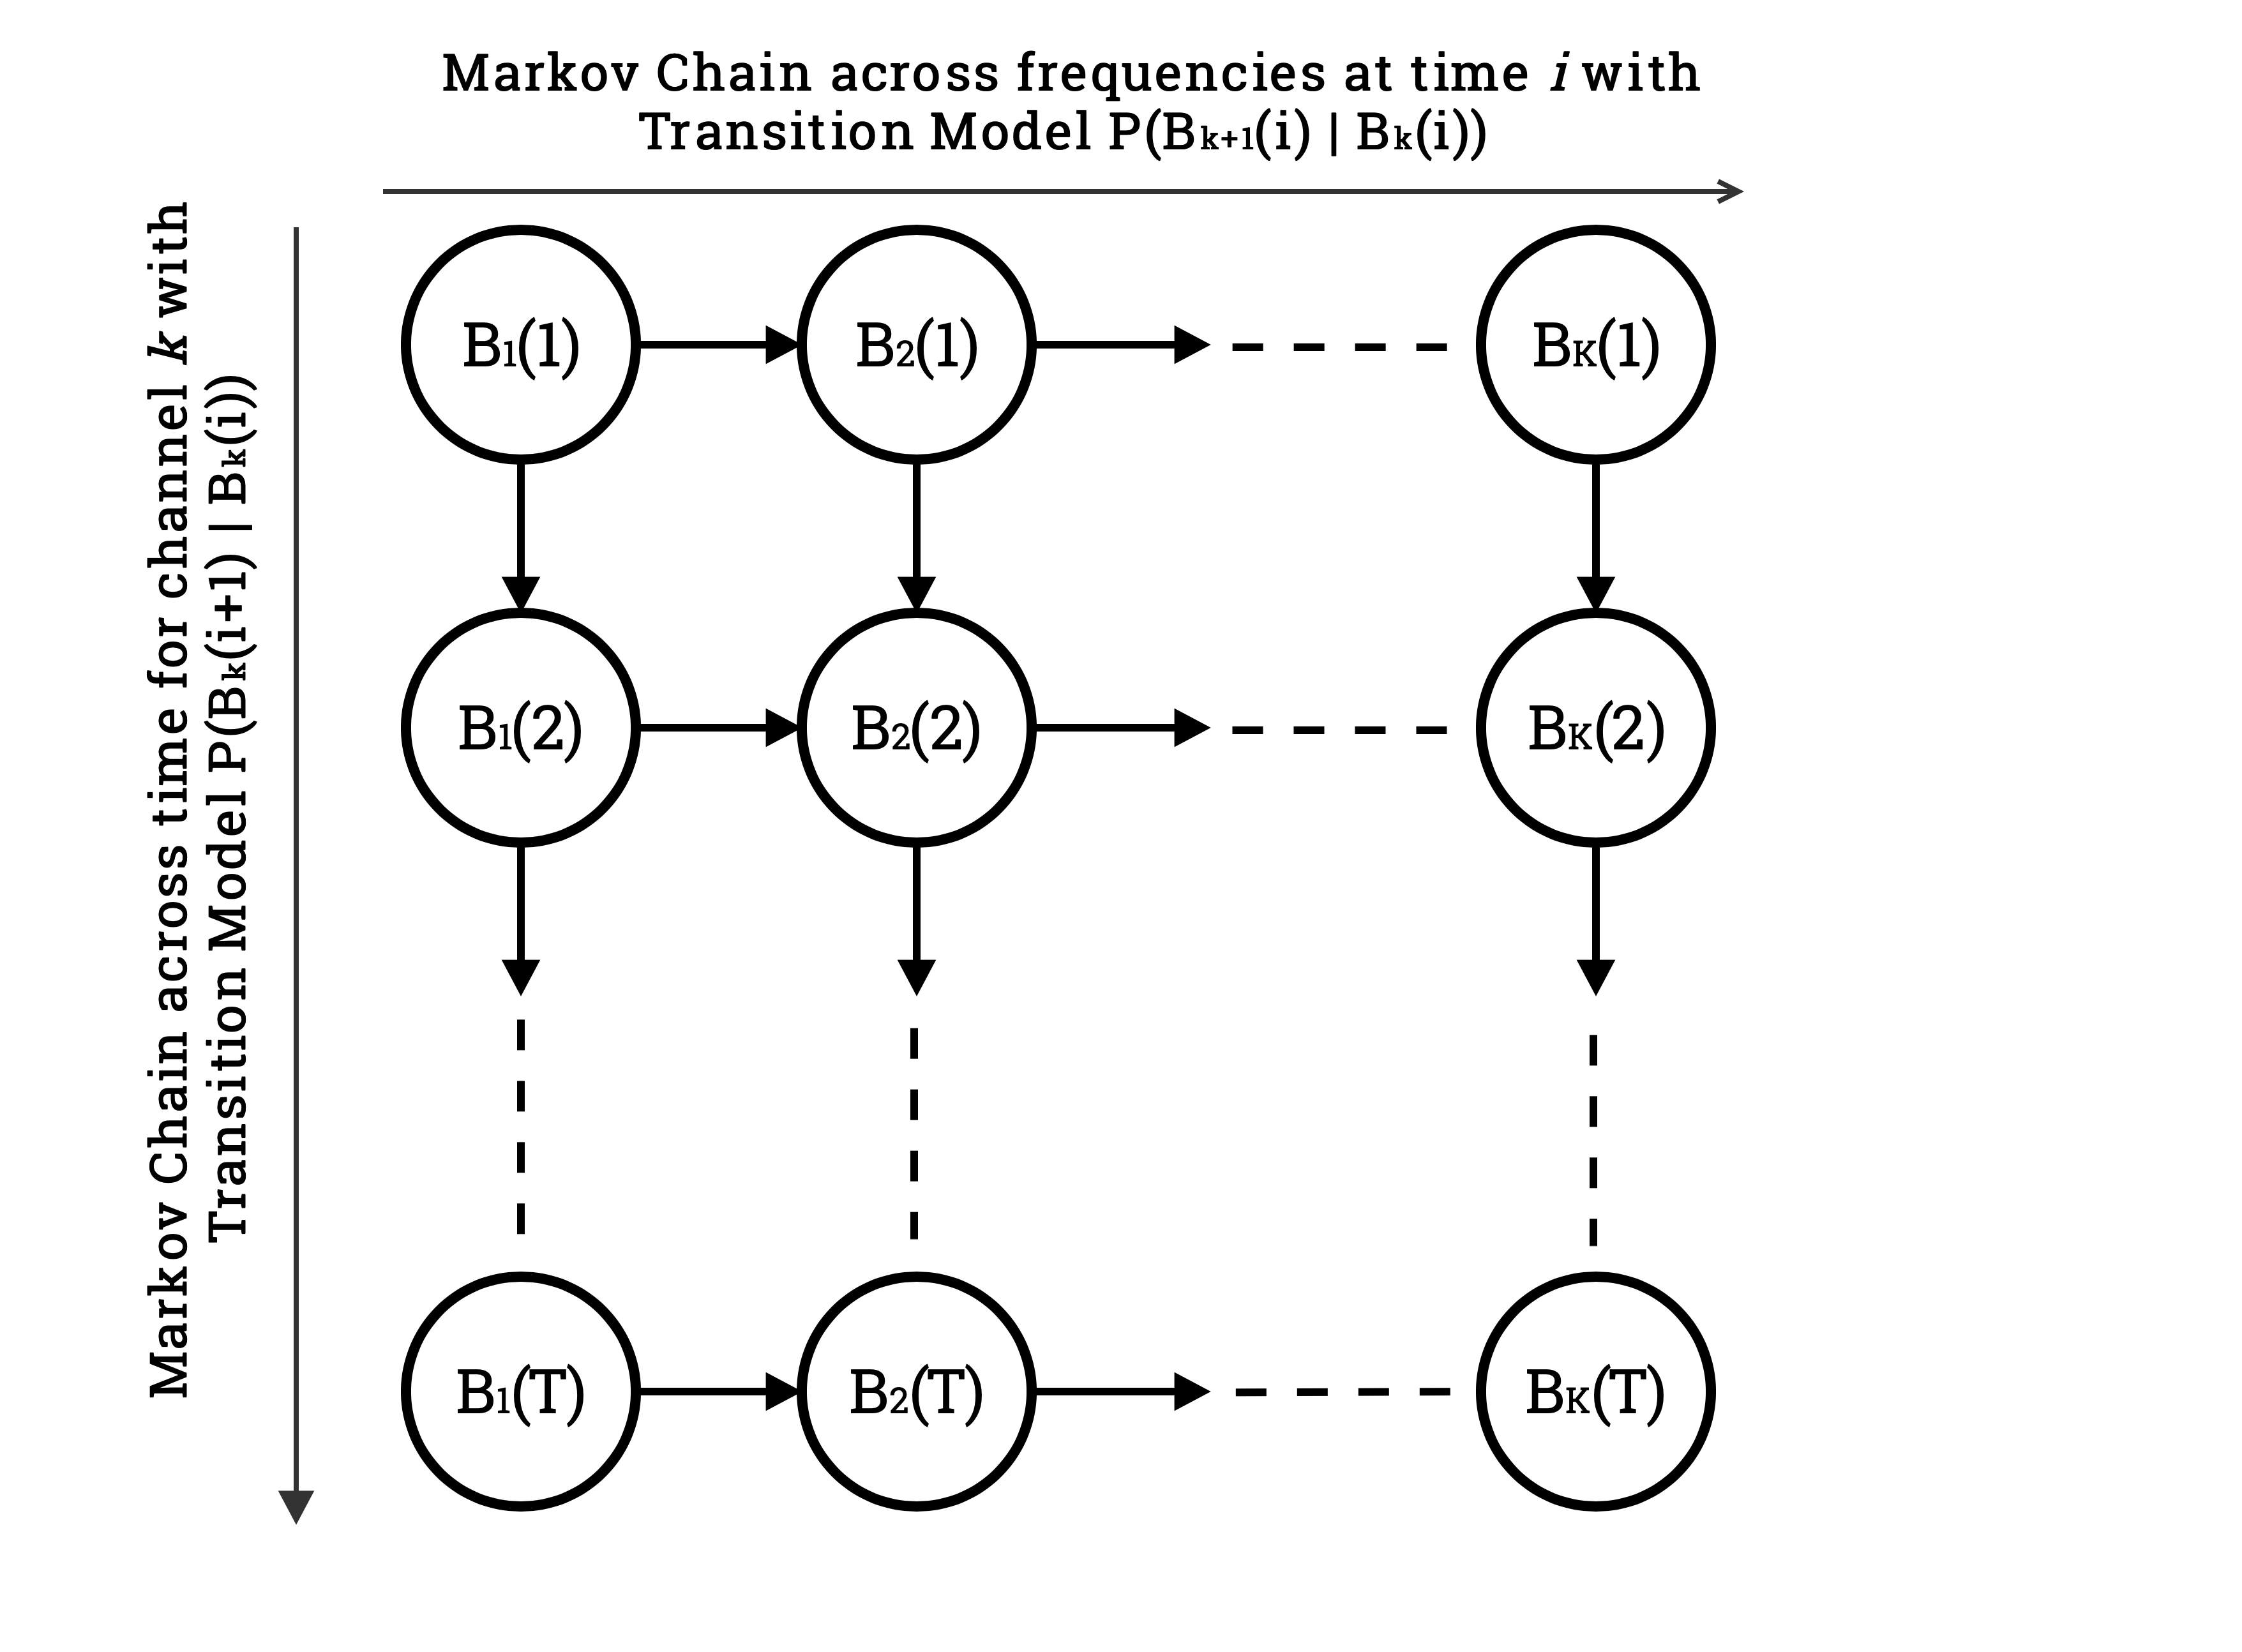
\includegraphics[width=0.75\linewidth]{MarkovChainsVisualization}
    \vspace{-5mm}
    \caption{The correlation model across time and frequencies underlying the occupancy behavior of incumbents in the network}
    \vspace{-5mm}
    \label{fig:1}
\end{figure}

\noindent {\bf PU Spectrum Occupancy Model:}
We\sst{ introduce the model of PU occupancy over time and across frequency by modeling each} \add{model} $X_k(i)$ as
\begin{equation}\label{4}
    X_k(i) = \sqrt{P_{tx}}B_k(i)S_k(i),
\end{equation}
where $P_{tx}$ is the transmission power of the PUs, $S_k(i)$ is the transmitted symbol modeled as a constant amplitude signal, $|S_k(i)|{=}1$, i.i.d. over time and across frequency bands;\footnote{\sst{In the case where}\add{If} $S_k(i)$ does not have constant amplitude, we may approximate $H_{k}(i)S_{k}(i)$ as complex Gaussian with zero mean and variance $\sigma_H^2\mathbb E[|S_{k}(i)|^2]$, without any modifications to the subsequent analysis.} $B_k(i){\in}\{0,1\}$ is the binary spectrum occupancy variable, with $B_k(i){=}1$, if the $k$th spectrum band is occupied by a PU at time $i$, and $B_k(i){=}0$, otherwise. Therefore, the PU occupancy\sst{ behavior} \add{state} in the entire wideband spectrum of interest at time $i$ can be modeled as the vector 
\begin{equation}\label{5}
    \vec{B}(i) = [B_1(i), B_2(i), B_3(i), \cdots, B_K(i)]^T {\in} \{0, 1\}^K.
\end{equation}
\sst{The }PUs join and leave the spectrum at random times. To capture this temporal correlation\sst{ in the spectrum occupancy dynamics of the PUs}, we model $\vec{B}(i)$ as a Markov process,
\begin{equation}\label{6}
    \begin{aligned}
        \mathbb{P}(\vec{B}(i+1)|\vec{B}(j), \forall j \leq i) = \mathbb{P}(\vec{B}(i+1)|\vec{B}(i)).
    \end{aligned}
\end{equation}
Additionally, when joining the spectrum pool, the PUs occupy a number of adjacent spectrum bands, and may vary their spectrum needs over time depending on time-varying traffic demands, channel conditions, etc. To capture this behavior, we model $\vec{B}(i)$ as a Markov chain across spectrum bands, i.e., the spectrum occupancy at time $i{+}1$ in frequency band $k$, $B_{k}(i{+}1)$, depends on the occupancy state of the adjacent spectrum band at the same time, $B_{k{-}1}(i{+}1)$, and that of the same spectrum band $k$ in the previous time index $i$, $B_{k}(i)$ as depicted in Fig. \ref{fig:1}, and described as
\begin{align}\label{7}
&         \mathbb{P}(\vec{B}(i+1)|\vec{B}(i))\\&=
\nonumber
         \mathbb{P}(B_{1}(i+1)|B_{1}(i))
         \prod_{k=2}^{K} \mathbb{P}(B_{k}(i+1)|B_{k}(i), B_{k-1}(i+1)).
\end{align}
Overall, we structure the correlation model as two Markov chains: one across time, parameterized by $q{=}\mathbb{P}(B_{k}(i{+}1){=}1|B_{k}(i){=}0)$, and the other across frequencies, parameterized by $p{=}\mathbb{P}(B_{k}(i{+}1){=}1|B_{k{-}1}(i{+}1){=}0)$. We estimate these parameters $p$ and $q$, using the parameter estimation algorithm described in Sec. \ref{III} in order to obtain the transition model underlying the MDP, given by \eqref{7}.

\noindent{\bf Spectrum Sensing Model:}
In order to detect the available spectrum holes, the SU performs spectrum sensing. However, owing to physical design limitations of its spectrum sensor \cite{5990482},\sst{ the SU} \add{it} can sense at most $\kappa$ out of $K$ spectrum bands at any given time, with $1{\leq}\kappa{\leq}K$. Let $\mathcal K_{i}{\subseteq}\{1,2,\dots,K\}$ with $|\mathcal K_i|{\leq}\kappa$ be the set of indices of spectrum bands sensed by the SU at time $i$, part of our design.
Then, we define the observation vector
\begin{equation}\label{8}
    \vec{Y}(i) = [Y_k(i)]_{k {\in} \mathcal K_i},
\end{equation}
\sst{where}\add{with} $Y_k(i)$\sst{ is} given by \eqref{3}.
The true states $\vec{B}(i)$ encapsulate the actual occupancy\sst{ behavior} \add{state} of the PUs, and the measurements $\vec{Y}(i)$ at the SU are noisy observations of these true states, which are modeled to be the observed states of an HMM. Given $\vec{B}(i)$ and $\mathcal K_i$, the probability density function of $\vec{Y}(i)$ is
\begin{equation}\label{9}
    f(\vec{Y}(i)|\vec{B}(i), \mathcal K_i) = \prod_{k \in \mathcal K_i} f(Y_k(i)|B_k(i)),
\end{equation}
owing to the independence of channels (given the occupancy states), noise, and transmitted symbols across frequency bands. Moreover, from \eqref{3},
\begin{equation}\label{10}
 Y_k(i)|B_k(i) \sim \mathcal{CN}(0, \sigma_H^2P_{tx}B_k(i) + \sigma_V^2).
\end{equation}

\noindent{\bf POMDP Agent Model:}
In this section, we model the SU as a POMDP agent, whose goal is to devise an optimal sensing and access policy in order to maximize its throughput, while ensuring minimal interference with incumbent transmissions. In fact, the agent's limited sensing capabilities coupled with its noisy observations result in an increased level of uncertainty\sst{ at the agent's end about} \add{on} the \add{PU spectrum occupancy state}\sst{ occupancy state of the spectrum under consideration} and \add{on} the exact effect of executing a\sst{n} \add{spectrum access} action on the radio environment. The transition model of the underlying MDP, as described by \eqref{7}, is denoted by $\mathbf{A}$ and is learned by the agent by interacting with the radio environment (see Sec. \ref{III}). The observation model is denoted by $\mathbf{M}$ and is given by \eqref{9}, with $f(Y_k(i)|B_k(i))$ given by \eqref{10}. 

We model the POMDP as a tuple $(\mathcal B,\mathcal{A},\mathcal{Y},\mathbf{A},\mathbf{M})$ where $\mathcal{B}{\equiv}\{0,1\}^K$ represents the state space of the underlying MDP, given by all possible realizations of the spectrum occupancy vector $\vec{B}$, as described by \eqref{5}; $\mathcal{A}$ represents the action space of the agent, given by all possible combinations in which $\kappa$ spectrum bands are chosen to be sensed out of $K$ at any given time; and $\mathcal{Y}$ represents the observation space of the agent based on the aforementioned signal model. The state of the POMDP at time $i$ is given by the \emph{prior belief} $\beta_i$, which represents the probability distribution of the underlying MDP state $\vec{B}(i)$, given the information collected by the agent up to time $i$, but before collecting the new information in time-step $i$. At the beginning of each time index $i$, given $\beta_i$, the agent selects $\kappa$ spectrum bands out of $K$, according to a policy $\pi(\beta_i)$, thus defining the sensing set $\mathcal K_i$, performs spectrum sensing  on these spectrum bands, observes $\vec{Y}(i){\in} \mathcal{Y}$, and updates its \emph{posterior belief} $\hat{\beta}_i$ of the current spectrum occupancy $\vec{B}(i)$ as 
\begin{align}\label{11}
\nonumber
\hat\beta_i(\vec{B}') &= \mathbb{P}(\vec{B}(i) = \vec{B}'|\vec{Y}(i), \mathcal K_i, \beta_i)\\&=
\frac{\mathbb{P}(\vec{Y}(i)|\vec{B}', \mathcal{K}_i) \beta_i(\vec{B}')}{
\sum_{\vec{B}'' {\in} \{0,1\}^K} \mathbb{P}(\vec{Y}(i)|\vec{B}'', \mathcal{K}_i) \beta_i(\vec{B}'')}.
\end{align}
We denote the function that maps the prior belief $\beta_i$ to the posterior belief $\hat\beta_i$ through the spectrum sensing action $\mathcal K_i$ and the observation signal $\vec{Y}(i)$ as $\hat\beta_i{=}\hat{\mathbb B}(\beta_i, \mathcal K_i, \vec{Y}(i))$.

Given the posterior belief $\hat{\beta}_i$, we estimate the occupancy state of the discretized spectrum under consideration as $\vec{B}(i)^{*}{=}\argmax_{\vec{B} {\in} \mathcal{B}} \hat{\beta}_{i}(\vec{B})$. Let $B_{k}(i)^{*}{=}\phi_{k}(\hat{\beta}_{i}) {\in} \{0, 1\}$ be the estimated state of channel $k$ at time $i$. If the channel is deemed to be idle as a result of this MAP estimation procedure, i.e., $\phi_{k}(\hat{\beta}_{i}){=}0$, the SU accesses the channel to deliver its network flows. Else, it leaves it untouched. Given the PU occupancy state $\vec{B}(i)$ and posterior belief $\hat\beta_i$, the reward metric of the POMDP is given by the number of \emph{truly idle} bands detected by the SU, accounting for the throughput maximization aspect of the agent's objective, and a penalty for \emph{missed detections} accounting for\sst{ the incumbent non-interference constraint} \add{interference to the incumbent},\sst{ i.e.,}
\begin{equation}
\nonumber
    R(\vec{B}(i), \hat{\beta}_i){=}\sum_{k=1}^{K} (1{-}B_k(i))(1{-}\phi_k(\hat{\beta}_{i})){-}\lambda B_k(i)(1 - \phi_k(\hat{\beta}_i)),
\end{equation}
where $\lambda{>}0$ represents a penalty factor. After performing data transmission, the SU computes the prior belief for the next time-step based on the dynamics of the Markov chain as
\begin{equation}\label{13}
    \beta_{i+1}(\vec{B}'')=\sum_{\vec{B}'}\mathbb{P}(\vec{B}(i+1) = \vec{B}''|\vec{B}(i)=\vec{B}')\hat{\beta}_{i}(\vec{B}').
\end{equation}
We denote the function that maps the posterior belief $\hat\beta_i$ to the prior belief $\beta_{i+1}$ as $\beta_{i+1}{=}{\mathbb B}(\hat\beta_i)$.
The goal\sst{ of the problem at hand} is to determine an optimal spectrum sensing policy to maximize the infinite-horizon discounted reward,
\begin{equation}\label{14}
    \pi^{*}{=}\argmax_{\pi} V^{\pi}(\beta) \triangleq \mathbb{E}_{\pi} \Big[\sum_{i=1}^{\infty} \gamma^{i} R(\vec{B}(i), \hat{\beta}_i)|\beta_0 {=}\beta\Big],
\end{equation}
where $0{<}\gamma{<}1$ is the discount factor, $\beta_0$ is the initial belief,\sst{ and} $\hat\beta_i$ is the posterior belief induced by policy $\mathcal K_i{=}\pi(\beta_i)$ and the observation $\vec{Y}(i)$ via $\hat\beta_i{=}\hat{\mathbb B}(\beta_i, \mathcal K_i, \vec{Y}(i))$, and we have defined the value function $V^{\pi}(\beta)$ under policy $\pi$ starting from belief $\beta$.
The optimal policy $\pi^*$ and the corresponding optimal reward $V^*(\beta)$ are the solutions of Bellman's optimality equation $V^*{=}\mathcal{H}[V^*]$, where the operator $V_{t+1}{=}\mathcal {H}[V_{t}]$ is defined as
\begin{align}\label{16}
\nonumber
        V_{t+1}(\beta) = &\max_{\mathcal{K} {\in} \mathcal{A}} \sum_{\vec{B} {\in} \mathcal{B}} \beta(\vec{B}) \mathbb{E}_{\vec{Y}|\vec{B}, \mathcal{K}} \Big[R(\vec{B}, \hat{\mathbb{B}}(\beta, \mathcal{K}, \vec{Y}))\\ &+\gamma V_{t}(\mathbb{B}(\hat{\mathbb{B}}(\beta, \mathcal{K}, \vec{Y})))\Big],\ \forall \beta.
\end{align}
This problem can be solved using the value iteration algorithm, i.e., by solving \eqref{16} iteratively until convergence to a fixed point. However, two challenges arise in our formulation:
\begin{itemize}
\item The correlation parameters $p$ and $q$ are unknown, hence the belief updates 
$\hat{\mathbb B}$ and $\mathbb B$ cannot be computed;
\item The number of states of the underlying MDP scales exponentially with the number of spectrum bands, resulting in a high-dimensional belief space, hence, solving equation \eqref{16} exactly is computationally infeasible.
\end{itemize}
To overcome these challenges, in the next section, we present a framework to estimate the transition model of the underlying MDP online, while concurrently utilizing this learned model to solve for the optimal policy\sst{ by employing} \add{via} PERSEUS, a low-complexity, randomized point-based value iteration algorithm \cite{DBLP:journals/corr/abs-1109-2145}.
\vspace{-6mm}
\section{Approaches and Algorithms}\label{III}
\noindent{\bf Occupancy Behavior\sst{ Transition} Model Estimation:}
In real-world implementations of cognitive radio\add{s}\sst{ systems}, the\sst{ mutable}\nm{mutable?}\sst{ transition model implicit in}
\add{correlation model defining} the occupancy behavior
 of the PUs is unknown to the SUs\sst{ in the network}, and therefore needs to be learned over time. The learned model then needs to be fed back to the POMDP agent which is solving for the optimal spectrum sensing and access policy simultaneously. Inherently, the approach constitutes solving the Maximum Likelihood Estimation (MLE) problem
\begin{equation}\label{17}
    \vec{\theta}^{*} = \argmax_{\vec{\theta}} \mathbb{P}([\vec{Y}(i)]_{i=1}^{\tau}|\vec{\theta}),
\end{equation}
where $\vec{\theta}{=}[p\ q]^{T}$, and $\tau$ refers to the learning period of the parameter estimator: this can be equal to the entire duration of the POMDP agent's interaction with the radio environment implying simultaneous model learning or can be a predefined parameter learning period before triggering the POMDP agent. Let $\add{\mathbf{Y}=}[\vec{Y}(i)]_{i{=}1}^{\tau}$\sst{ be denoted as as $\mathbf{Y}$} and $\add{\mathbf{B}=}[\vec{B}(i)]_{i{=}1}^{\tau}$\sst{ as $\mathbf{B}$}. Re-framing \eqref{17} as an optimization of the log-likelihood, we get\sst{,}
\begin{equation}\label{18}
    \vec{\theta}^{*} = \argmax_{\vec{\theta}} \log\Big(\sum_{\mathbf{B}} \mathbb{P}(\mathbf{B}, \mathbf{Y}| \vec{\theta})\Big).
\end{equation}
This problem can be solved using the Expectation-Maximization (EM) algorithm \cite{778361}, with the E-step given by
\begin{equation}
    Q(\vec{\theta}|\vec{\theta}^{(t)}) = \mathbb{E}_{\mathbf{B}|\mathbf{Y}, \vec{\theta}^{(t)}} \Big[ \log \Big(\sum_{\mathbf{B}} \mathbb{P}(\mathbf{B}, \mathbf{Y}|\vec{\theta}^{(t)})\Big)\Big].
\end{equation}
This can be obtained by employing the Forward-Backward algorithm \cite{778361} using the current estimate $\vec{\theta}^{(t)}$. The M-step constitutes
\begin{equation}
\vec{\theta}^{(t+1)}
 = \argmax_{\vec{\theta}} Q(\vec{\theta}|\vec{\theta}^{(t)}),
\end{equation}
which involves re-estimation of the maximum likelihood parameters in $\vec{\theta}$ using the statistics obtained from the Forward-Backward algorithm.

\noindent{\bf The PERSEUS Algorithm:}
We solve for the optimal spectrum sensing and access policy, formulated as a POMDP, in parallel with the parameter estimation algorithm, employing the model estimates until both the EM and the POMDP algorithms converge. As discussed in Sec. \ref{II} of this article, solving the Bellman equation \eqref{16} for POMDPs with large state and action spaces using exact value iteration\sst{ and policy iteration methods} is computationally infeasible \cite{DBLP:journals/corr/abs-1109-2145}. Hence, we resort to approximate value iteration methods to ensure that the system scales well to a large number of bands in the spectrum of interest. One such method, the PERSEUS algorithm \cite{DBLP:journals/corr/abs-1109-2145} is a randomized point-based approximate value iteration technique that involves an initial phase of determining a set of so-called \emph{reachable beliefs} $\tilde{\mathcal{B}}$ by allowing the agent to randomly interact with the radio environment. The goal of\sst{ the} PERSEUS\sst{ algorithm} is to improve the value of all the belief points in this set $\tilde{\mathcal{B}}$ by updating the value of only a subset of these belief points, chosen iteratively at random. Using the notion that, for finite-horizon POMDPs, $V^*$ in \eqref{16} can be approximated by a piece-wise linear and convex function \cite{DBLP:journals/corr/abs-1109-2145},\sst{ the} PERSEUS\sst{ algorithm} operates on the core idea that the value function at iteration $t$ can be parameterized by a set of hyperplanes $\{\vec{\alpha}_{t}^{u}\}$, $u {\in} \{1,2,\dots,|\tilde{\mathcal{B}}|\}$, each representing a region of the belief space for which it is the maximizing element, and each associated with an optimal spectrum sensing action $\mathcal K_t^{u}$. That is, when operating with belief $\beta$, the value function is approximated as
\begin{equation}
    \begin{aligned}\label{40}
        V_{t}(\beta) \approx \beta \cdot \vec{\alpha}_{t}^{u^*},
        \ 
        u^* = \argmax_{u\in\{1,2,\dots,|\tilde{\mathcal{B}}|\}} \beta \cdot \vec{\alpha}_{t}^{u},
    \end{aligned}
\end{equation}
and the optimal spectrum sensing action is $\mathcal K_t^{u^*}$, where $\beta\cdot\vec{\alpha}{=}\sum_{\vec{B}}\beta(\vec{B})\vec{\alpha}(\vec{B})$
 denotes inner product. The set of hyperplanes $\{\vec{\alpha}_{t}^{u}\}$ associated with the set $\tilde{\mathcal{B}}$ are\sst{ to be} improved over\sst{ numerous} \add{multiple} iterations of PERSEUS\sst{.
  Specifically,}\add{:} given $\{\vec{\alpha}_{t}^{u}\}$ and the optimal spectrum sensing actions
$\{\mathcal K_{t}^{u}\}$ at iteration $t$, a PERSEUS iteration generates a new set of hyperplanes $\{\vec{\alpha}_{t+1}^{u}\}$ and associated spectrum sensing actions
$\{\mathcal K_{t+1}^{u}\}$, as we now describe. Let $\tilde{\mathcal{U}}$ be the set of unimproved belief points (initially, $\tilde{\mathcal{U}}{=}\tilde{\mathcal{B}}$). Then, a belief $\beta_u$ is picked randomly from $\tilde{\mathcal{U}}$. Next, a \emph{backup} operation is performed on $\beta_u$ to determine a new associated hyperplane and spectrum sensing action as \cite{DBLP:journals/corr/abs-1109-2145}
\begin{equation}\label{20}
    \vec{\alpha}_{t+1}^{u}=\Xi_{\mathcal K_{t+1}^{u}}^{u},\ 
    \mathcal K_{t+1}^{u}=\argmax_{\mathcal{K} \in \mathcal{A}} \beta_u \cdot \Xi_{\mathcal{K}}^{u},
\end{equation}
where $\Xi_{\mathcal{K}}^{u}$ is the hyperplane corresponding to a one-step look-ahead under action $\mathcal K$ and belief $\beta_u$, given by
\begin{align*}
\Xi_{\mathcal{K}}^{u}(\vec{B}) = &\mathbb{E}_{\vec{Y}|\vec{B}, \mathcal{K}} \Big[R(\vec{B}, \hat{\mathbb{B}}(\beta_{u}, \mathcal{K}, \vec{Y}))\\
&+\gamma 
        \sum_{\vec{B}'}\mathbb{P}(\vec{B}(i+1){=} \vec{B}'|\vec{B}(i){=}\vec{B})
                \Xi_{\mathcal{K}, \vec{Y}}^{u}(\vec{B}')\mid\vec{B}\Big]
\nonumber
\end{align*}
and $\Xi_{\mathcal{K}, \vec{Y}}^{u}$ is the hyperplane associated with the future value function computed from the previous set of hyperplanes as
\begin{equation}
    \Xi_{\mathcal{K}, \vec{Y}}^{u}=\argmax_{\alpha_{t}^{u'}, u' {\in} \{1, 2, \dots, |\tilde{\mathcal{B}}|\}} \mathbb{B}(\hat{\mathbb{B}}(\beta_{u}, \mathcal{K}, \vec{Y}))\cdot\alpha_{t}^{u'},
\nonumber
\end{equation}
under the new belief $\mathbb{B}(\hat{\mathbb{B}}(\beta_{u}, \mathcal{K}, \vec{Y}))$ reached from $\beta_{u}$, under action $\mathcal{K}$ and observation $\vec{Y}$, in one step. At this point, $\beta_{u}{\cdot}\vec{\alpha}_{t+1}^{u}$ is the approximate value function associated with the belief $\beta_u$. If $\beta_{u}{\cdot}\vec{\alpha}_{t+1}^{u}{\geq}V_{t}(\beta_{u})$, the newly defined hyperplane generates an improved value function; otherwise ($\beta_{u}{\cdot}\vec{\alpha}_{t+1}^{u}{<}V_{t}(\beta_{u})$), the value function is worsened and the previous hyperplane is kept, hence $\vec{\alpha}_{t+1}^{u}{:=}\vec{\alpha}_{t}^{u}$ and $\mathcal K_{t+1}^{u}{:=}\mathcal K_{t}^{u}$. Finally, the belief $\beta_u$ is removed from $\tilde{\mathcal{U}}$, along with all belief points that are improved by the newly added hyperplane:
$$
\tilde{\mathcal{U}}\leftarrow \tilde{\mathcal{U}}\setminus\{\beta_u\}\setminus
\{\beta'\in\tilde{\mathcal{U}}:\beta'{\cdot}\vec{\alpha}_{t+1}^{u}\geq V_t(\beta')\}.
$$
This operation continues until the set $\tilde{\mathcal{U}}$ is empty. The PERSEUS iterations continue until the number of policy changes between consecutive iterations is below a specified threshold $\eta$. The belief update procedure outlined in \eqref{11} is an essential aspect of POMDPs, which can turn into a performance bottleneck for large state spaces due to the inherent iteration over all possible states. In order to circumvent this problem, we fragment the spectrum into smaller, independent sets of correlated channels and then run the PERSEUS algorithm on these fragments by leveraging multi-processing and multi-threading tools available at our disposal in software frameworks. Furthermore, we avoid iterating over all possible states and allow only those state transitions we deem to be the most probable -- for example, only those state transitions that involve a Hamming distance of up to $3$ between the previous and current state vectors in a radio environment with $18$ frequency channels.
\vspace{-4mm}
\section{Numerical Evaluations}\label{IV}
\nm{please let us agree on the mathematical part before you finalize the numerical results...}
\noindent{\bf Simulation Setup:}
We simulate a radio environment with $J{=}3$ PUs occupying a set of $K{=}18$ channels, each of bandwidth $\text{BW}_{k}{=}160 \text{kHz}$, according to a Markovian time-frequency correlation structure defined by the parameters $p{=}q{=}0.3$, and a\sst{n} SU intelligently trying to access the available white spaces. Considering a noise spectral density of $N_0{=}{-}22 \text{dBm/Hz}$, we set $\sigma_V^2{=}1$ for the noise variance. Furthermore, we set $\sigma_{H}^{2}{=}80$ for the Rayleigh fading variance, $P_{tx,j}{=}64.771 \text{dBm}$\nm{you don't need all thes digits..65 is fine} for the transmit power of PU $j$, and $\tilde{P}_{tx}{=}54.771 \text{dBm}$\nm{you don't need all thes digits..55 is fine} for the transmit power of the SU. Simulating a typical power-law propagation model with a path-loss exponent of $\nu{=}1.5$\nm{isn't PLE typically larger than 2? In addition, the experience SNR depends on distance.. what is the distance?}, the SINR at incumbent $j$ with respect to channel $k$ at time $i$ is $\text{SINR}_{\text{PU}_{j},k}(i){=}17.386 \text{dB}$\nm{you don't need all thes digits..17 is fine} when there is no interference from the SU, and $\text{SINR}_{\text{PU}_{j},k}'(i){=}4.756 \text{dB}$\nm{you don't need all thes digits..5 is fine} with SU interference. Similarly, the SINR at the SU with respect to channel $k$ at time $i$ is $\text{SINR}_{\text{SU},k}(i){=}12.386 \text{dB}$\nm{you don't need all thes digits..12 is fine} when the channel is truly idle, and $\text{SINR}_{\text{SU},k}'(i){=}{-}5.078 \text{dB}$\nm{you don't need all thes digits..-5 is fine} when the channel is occupied by an incumbent. Assuming that the SU is always backlogged, each channel $k$ offers a maximum AWGN throughput\nm{what do you mean by max AWGN throughput?} of $C_{\text{max},k}^{\text{SU}}(i){=}\text{BW}_{k}\log_{2}(1{+}\text{SINR}_{\text{SU},k}(i)){=}0.671$Mbps for the SU, when the channel is truly idle at time $i$; and PU $j$ achieves a maximum AWGN throughput of $C_{\text{max},k}^{\text{PU}_{j}}(i){=}\text{BW}\log_{2}(1{+}\text{SINR}_{\text{PU}_{j}, k}(i)){=}0.928$Mbps, when there is no interference from the SU on channel $k$ at time $i$. Subject to the Rayleigh fading model detailed in Sec. \ref{II}, the expected throughput can evaluated as $$C_{k}(i) = \int_{0}^{\infty}\text{BW}_{k}\log_{2}(1+\phi)f_{\Phi}(\phi)d\phi,$$ where $\phi$ is the fading SINR, and $f_{\Phi}(\phi)$ is the distribution of the fading SINR. Using this result, the expected throughput for the SU is found to be $C_{k}^{\text{SU}}(i){=}0.512$Mbps, when channel $k$ is truly idle at time $i$; and the expected throughput for incumbent $j$ on channel $k$ at time $i$ is found to be $C_{k}^{\text{PU}_{j}}(i){=}0.643$Mbps, when there is no SU interference. We further assume that the SU accesses all channels that are deemed idle by the POMDP agent in any given time-step $i$, thereby giving us an SU throughput metric described as $$C^{\text{SU}}{=}\sum_{k=1}^{K}(1{-}B_{k}(i))(1{-}\phi_{k}(\hat{\beta}_{i}))C_{k}^{\text{SU}}(i)\ \text{Mbps}.$$
\nm{why do you need both $C_{\text{max},k}$ and this integral expression?
I would make it more precise as follows: the PU transmits at a certain rate R.. if 
$R>C_{k}(SINR)$ (capacity under current SINR, which is a random variable since it includes fading) then tx fails. Otherwise, it succeeds. Hence the throuhgput is
$$
R\cdot\mathbb P(R\leq B\log_2(1+SINR))
=
R\cdot\mathbb P(SINR\geq 2^{R/B}-1)
$$
which can be easily computed in closed form since SINR is exponential rv. Please fix and finish the steps.}
 Additionally, estimating that the expected throughput for incumbent $j$ is $C{'}_{k}^{\text{PU}_{j}}(i){=}0.370$Mbps when the SU also accesses channel $k$ at time $i$, we evaluate PU interference by defining an indicator variable $\mathcal{I}$ which is assigned a value of $1$ when the throughput at PU $j$ with respect to channel $k$, at a given time-step $i$, drops to or below $0.370$Mbps, thereby giving us a normalized interference metric with respect to all $J$ PUs and $K$ channels as $$I = \mathbb{E}_{i}\left[\frac{\sum_{j}\sum_{k}B_{j,k}(i)\mathcal{I}(C_{k}^{\text{PU}_{j}}(i){\leq}0.370 \text{Mbps})}{\sum_{k}B_{k}(i)}\right].$$
 \nm{why not simply computing the PU throughput as I have defined above? I.e.
 $$\sum_kR\cdot\mathbb P(SINR_k\geq 2^{R/B}-1)$$
 where $SINR_k$ is an exponential rv with mean dependent on whether SU is idle or transmits...}
We impose a sensing restriction on the SU: at most $\kappa{=}6$ out of $K{=}18$ channels can be sensed by the SU in any given time-step $i$. Finally, while solving for the optimal policy in the PERSEUS algorithm, we employ a discount factor of $\gamma{=}0.9$ and a termination threshold of $\eta{=}0$.

\noindent{\bf Evaluations:}
The plot depicted in Fig. \ref{fig:4} shows the mean square error (MSE) convergence of the parameter estimation algorithm to determine the parametric time-frequency correlation structure, i.e., $p$ and $q$. Starting with an initial estimate of $10^{-8}$, the EM algorithm iteratively reduces the MSE given by $\mathbb{E}[(\theta_{i}{-}\hat{\theta}_{i}^{(t)})^{2}],\ \theta_{i}{\in}[p,q]^{\intercal}$, as it goes through the E and M steps, and converges to the true transition model with an error of $\epsilon{\leq}10^{-8}$ over approximately $24000$ iterations. Since the EM algorithm is susceptible to premature convergence to local optima and saddle points, we mitigate this by averaging the procedure over several cycles.
\begin{figure}
    \centering
    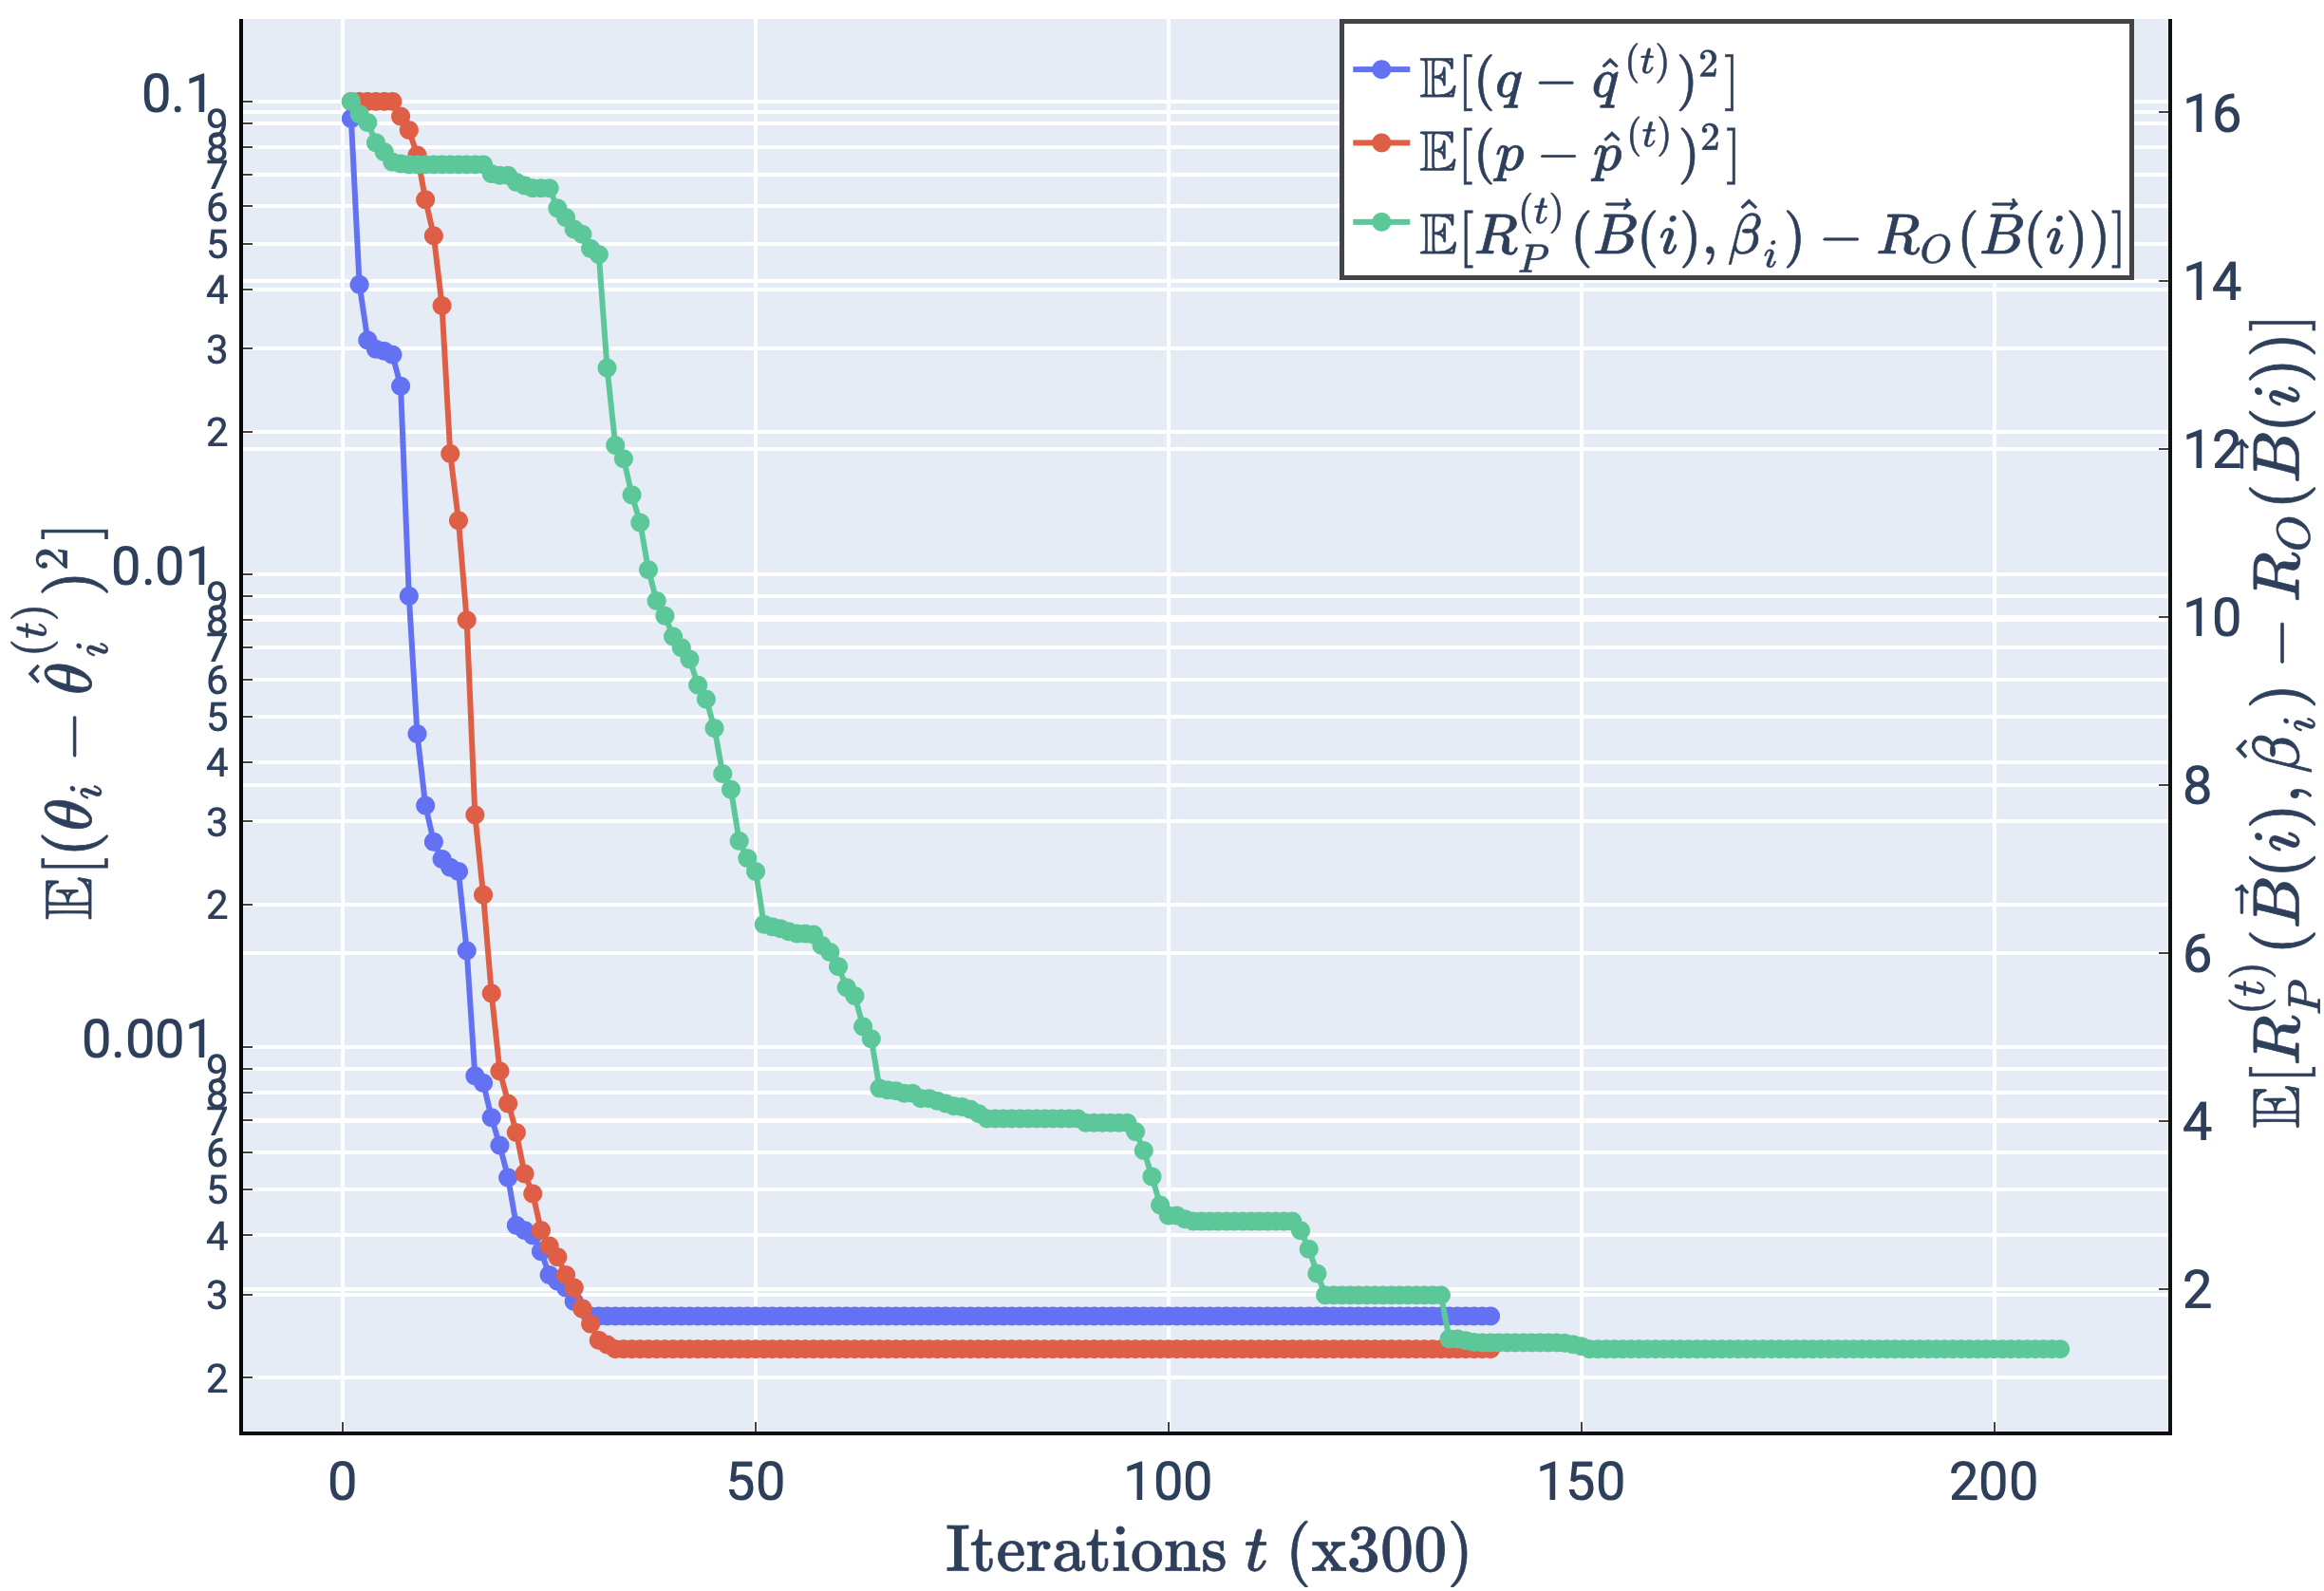
\includegraphics[width=0.75\linewidth]{PerseusRegretConvergence_MeanSquareErrorConvergence.png}
    \caption{MSE convergence of the parameter estimation algorithm while determining the correlation models $p$ and $q$, and the Regret convergence of the fragmented PERSEUS algorithm with belief simplification}
    \vspace{-4mm}
    \label{fig:4}
\end{figure}
Fig. \ref{fig:4} also illustrates the \emph{Regret} convergence plot of the PERSEUS algorithm, on the same time scale and in the same simulation run, over several iterations $t$, wherein the regret metric corresponds to the difference in utility obtained by our PERSEUS algorithm at a certain iteration $t$ in our simulation, denoted by $R_{P}^{(t)}(\vec{B}(i), \hat{\beta}_{i})$, and an \emph{Oracle} which has complete information about the occupancy behavior of incumbents in the network, whose utility is denoted by $R_{O}(\vec{B}(i))$. This trace in Fig. \ref{fig:4}, similar to the \emph{Reward v/s Time} plot in \cite{DBLP:journals/corr/abs-1109-2145}, serves as a measure of convergence for our fragmented PERSEUS algorithm with simplified belief updates and online model estimation.

We evaluate the performance of the proposed framework in terms of the SU network throughput and PU interference metrics over varying values of the penalty term $\lambda$ as illustrated in Fig. \ref{fig:8}. As surmised, we find that our POMDP agent decides to limit channel access when the penalty is high, leading to lower SU network throughput and lower PU interference; and on the other hand, it follows a more lenient channel access strategy when the penalty is low, resulting in higher SU network throughput and higher PU interference. In general, we observe the trend of rising throughput and increasing interference as the penalty for missed detections $\lambda$ is lowered. Comparing this performance of our proposed framework with correlation-coefficient based state-of-the-art, namely the Minimum Entropy Merging (MEM) with Minimum Entropy Increment (MEI) Channel Correlation Estimation (CCE) and Markov Process Estimation (MPE) algorithm with a correlation threshold of $\rho_{th}{=}0.77$ and $6$ specified clusters, from \cite{6956794}, we find that our framework achieves higher SU network throughput and lower PU interference with $\lambda{\geq}10$. Furthermore, the proposed framework comes very close to achieving the throughput attained by a Viterbi agent \cite{4554696}, while providing the same interference performance. It is worth noting that the Viterbi agent possesses prior knowledge about the transition model of the underlying MDP and senses more channels per time-step than our POMDP agent. More importantly, unlike these other works, the proposed framework allows us to regulate the trade-off between the interference caused to PUs and the throughput of the SU, by adjusting the parameter $\lambda$.
\vspace{-4mm}
\section{Conclusion}\label{V}
\begin{figure}
    \centering
    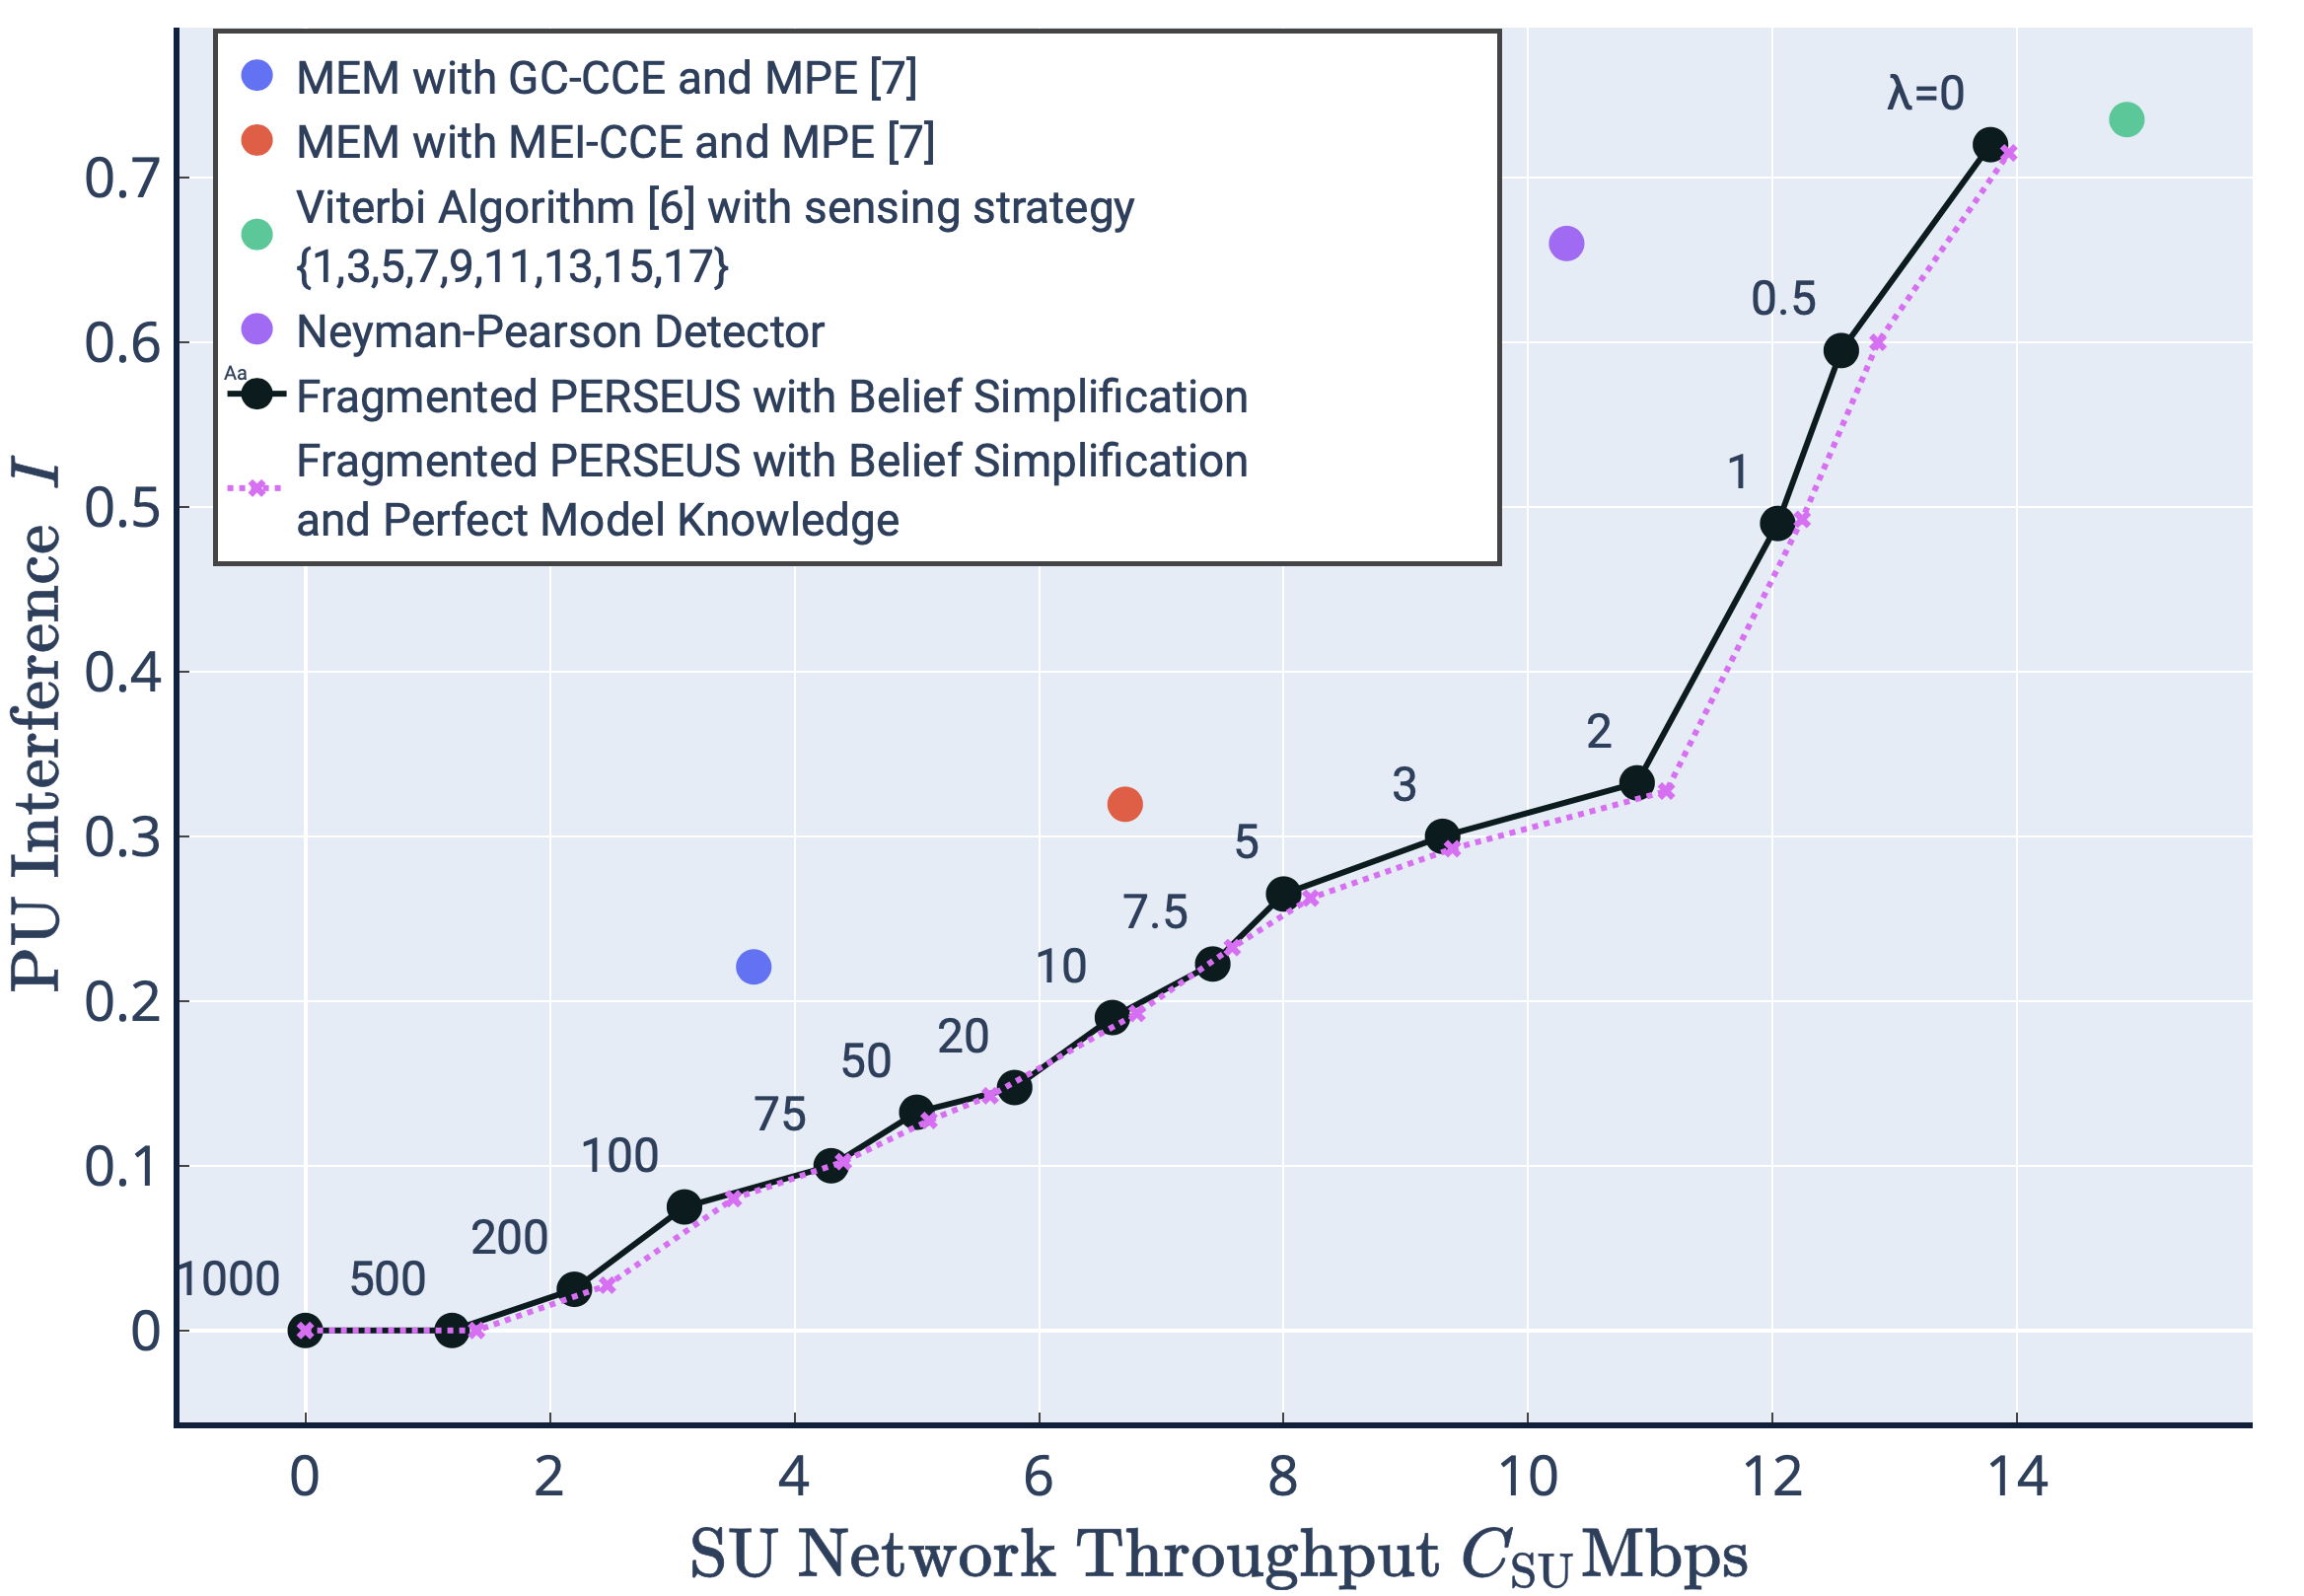
\includegraphics[width=0.75\linewidth]{SU_Throughput_PU_Interference_Varying_Penalty.png}
    \caption{SU Network Throughput versus PU Interference evaluation of the proposed framework over varying values of the penalty $\lambda$}
    \vspace{-5mm}
    \label{fig:8}
\end{figure}
In this letter, we formulate the optimal spectrum sensing and access problem in an AWGN observation model with multiple licensed users and a cognitive radio restricted in terms of its sensing capabilities, as a POMDP. In a radio environment wherein the occupancy behavior of the incumbents is correlated across time and frequencies, we present a consolidated framework that employs the EM algorithm to estimate the transition model of this occupancy behavior, and leverage a fragmented PERSEUS algorithm with belief update heuristics to simultaneously solve for the optimal spectrum sensing and access policy. Through system simulations, we conclude that our framework, in addition to its superior performance compared to algorithms in the state-of-the-art, facilitates regulation of the trade-off between SU throughput and PU interference.
\bibliographystyle{IEEEtran}
\vspace{-8mm}
\bibliography{ref}
\end{document}